\documentclass[14pt,a4paper]{extarticle}
% =============================================================
% preamble.tex — Shared LaTeX preamble for genetic/evolutionary reports
% Conforming to BSUIR STP 01-2024
% =============================================================

% Encoding and language
\usepackage[utf8]{inputenc}
\usepackage[T2A]{fontenc}
\usepackage[russian]{babel}

% Times New Roman font
\usepackage{tempora}

% Page geometry: STP 2.1.1
\usepackage{geometry}
\geometry{left=30mm, right=15mm, top=20mm, bottom=20mm}

% Line spacing: STP 2.1.1
\usepackage{setspace}
\singlespacing

% Allow TeX a bit more flexibility to avoid overflow
\pretolerance=1000
\tolerance=2000
\emergencystretch=3em

% Paragraph indent
\usepackage{indentfirst}
\setlength{\parindent}{1.25cm}

% Page numbers
\usepackage{fancyhdr}
\pagestyle{fancy}
\fancyhf{}
\fancyfoot[R]{\thepage}
\renewcommand{\headrulewidth}{0pt}
\fancypagestyle{plain}{%
  \fancyhf{}%
  \fancyfoot[R]{\thepage}%
  \renewcommand{\headrulewidth}{0pt}%
}

% Math
\usepackage{amsmath,amssymb}

% Graphics
\usepackage{graphicx}
\usepackage{float}
\usepackage{xcolor}

% Tables
\usepackage{booktabs}
\usepackage{tabularx}
\usepackage{multirow}
\usepackage{longtable}

% Captions
\usepackage{caption}
\captionsetup[figure]{
  labelsep=endash,
  justification=centering,
  font={normalsize},
  name=Рисунок
}
\captionsetup[table]{
  labelsep=endash,
  justification=raggedright,
  singlelinecheck=false,
  font={normalsize},
  name=Таблица
}

% Section formatting
\usepackage{titlesec}
\titleformat{\section}
  {\newpage\normalfont\fontsize{14}{18}\selectfont\bfseries}
  {\thesection}{0.5em}{\MakeUppercase}
\titlespacing*{\section}{1.25cm}{0pt}{14pt}

\titleformat{\subsection}
  {\normalfont\fontsize{14}{18}\selectfont\bfseries}
  {\thesubsection}{0.5em}{}
\titlespacing*{\subsection}{1.25cm}{14pt}{14pt}

\titleformat{\subsubsection}
  {\normalfont\fontsize{14}{18}\selectfont\bfseries}
  {\thesubsubsection}{0.5em}{}
\titlespacing*{\subsubsection}{1.25cm}{14pt}{14pt}

% Unnumbered sections
\newcommand{\sectioncenter}[1]{%
  \newpage
  \phantomsection
  \addcontentsline{toc}{section}{#1}
  \begin{center}
    \textbf{\MakeUppercase{#1}}
  \end{center}
  \vspace{14pt}
}

% Table of contents formatting
\usepackage{tocloft}
\renewcommand{\cftsecfont}{\normalfont}
\renewcommand{\cftsecpagefont}{\normalfont}
\renewcommand{\cftsubsecfont}{\normalfont}
\renewcommand{\cftsubsecpagefont}{\normalfont}
\renewcommand{\cftsecleader}{\cftdotfill{\cftdotsep}}
\renewcommand{\cftdotsep}{1}
\renewcommand{\contentsname}{\hfill\textbf{СОДЕРЖАНИЕ}\hfill}
\renewcommand{\cftaftertoctitle}{\hfill}

% Lists
\usepackage{enumitem}
\setlist[itemize]{noitemsep, topsep=0pt, leftmargin=1.25cm, label=--}
\setlist[enumerate]{noitemsep, topsep=0pt, leftmargin=1.25cm}

% Code listings
\usepackage{listings}
\usepackage{fancyvrb}
\lstset{
  basicstyle=\ttfamily\small,
  frame=single,
  breaklines=true,
  showstringspaces=false,
  inputencoding=utf8,
  extendedchars=true,
  literate={а}{{\cyra}}1 {б}{{\cyrb}}1 {в}{{\cyrv}}1 {г}{{\cyrg}}1
           {д}{{\cyrd}}1 {е}{{\cyre}}1 {ж}{{\cyrzh}}1 {з}{{\cyrz}}1
           {и}{{\cyri}}1 {й}{{\cyrishrt}}1 {к}{{\cyrk}}1 {л}{{\cyrl}}1
           {м}{{\cyrm}}1 {н}{{\cyrn}}1 {о}{{\cyro}}1 {п}{{\cyrp}}1
           {р}{{\cyrr}}1 {с}{{\cyrs}}1 {т}{{\cyrt}}1 {у}{{\cyru}}1
           {ф}{{\cyrf}}1 {х}{{\cyrh}}1 {ц}{{\cyrc}}1 {ч}{{\cyrch}}1
           {ш}{{\cyrsh}}1 {щ}{{\cyrshch}}1 {ъ}{{\cyrhrdsn}}1
           {ы}{{\cyrery}}1 {ь}{{\cyrsftsn}}1 {э}{{\cyrerev}}1
           {ю}{{\cyryu}}1 {я}{{\cyrya}}1
}

% Hyperlinks
\usepackage{hyperref}
\hypersetup{
  colorlinks=true,
  linkcolor=black,
  urlcolor=blue,
  citecolor=black,
}

% Number figures and tables within sections
\numberwithin{figure}{section}
\numberwithin{table}{section}
\numberwithin{equation}{section}

% Standard title page macro
\newcommand{\makegeclabtitle}[2]{%
  \begin{titlepage}
  \thispagestyle{empty}
  \begin{center}

  МИНИСТЕРСТВО ОБРАЗОВАНИЯ РЕСПУБЛИКИ БЕЛАРУСЬ

  \vspace{0.5em}

  Учреждение образования

  \vspace{0.5em}

  \textbf{<<Белорусский государственный университет информатики и радиоэлектроники>>}

  \vspace{2em}

  Факультет компьютерных систем и сетей

  \vspace{0.5em}

  Кафедра программного обеспечения информационных технологий

  \end{center}

  \vspace{3em}

  \begin{center}
  \textbf{ОТЧЕТ}

  \vspace{0.5em}

  по лабораторной работе №#1

  \vspace{0.5em}

  по дисциплине

  \vspace{0.5em}

  <<Генетические и эволюционные вычисления>>

  \vspace{0.5em}

  <<#2>>
  \end{center}

  \vspace{5em}

  \begin{flushright}
  \begin{minipage}{0.5\textwidth}
  \textbf{Выполнил:}\\
  Лебедевич Артем Владимирович\\
  магистрант группы 556301

  \vspace{0.6em}

  \textbf{Преподаватель:}\\
  Нестеренков Сергей Николаевич\\
  кандидат технических наук\\
  доцент кафедры ПОИТ
  \end{minipage}
  \end{flushright}

  \vfill

  \begin{center}
  Минск, 2026~г.
  \end{center}

  \end{titlepage}
}

\graphicspath{{figures/}}

\begin{document}

\makegeclabtitle{1}{Классификация с помощью персептрона}

\tableofcontents

\newpage

\section{Цель работы}

Изучить принципы работы персептрона для решения задач классификации. Реализовать однослойный персептрон с одним и двумя нейронами, продемонстрировать его возможности и ограничения на задачах бинарной и многоклассовой классификации.

\section{Теоретические сведения}

\subsection{Персептрон}

Персептрон~--- это простейшая модель искусственного нейрона, предложенная Ф.~Розенблаттом в 1958~г. Персептрон с $n$ входами вычисляет взвешенную сумму входных сигналов и применяет к ней пороговую функцию активации:

\begin{equation}
y = f\left(\sum_{i=1}^{n} w_i x_i + b\right),
\end{equation}

где $w_i$~--- веса, $b$~--- смещение (bias), а $f$~--- функция активации (ступенчатая функция Хевисайда):

\begin{equation}
f(z) = \begin{cases} 1, & z \geq 0, \\ 0, & z < 0. \end{cases}
\end{equation}

\subsection{Алгоритм обучения персептрона}

Обучение персептрона происходит итеративно по правилу:
\begin{equation}
w_i^{(t+1)} = w_i^{(t)} + \eta \cdot (d - y) \cdot x_i,
\end{equation}
\begin{equation}
b^{(t+1)} = b^{(t)} + \eta \cdot (d - y),
\end{equation}

где $\eta$~--- скорость обучения, $d$~--- целевое значение, $y$~--- выход персептрона.

Согласно теореме о сходимости персептрона, если данные линейно разделимы, алгоритм гарантированно сходится за конечное число итераций.

\subsection{Проблема XOR}

Персептрон способен разделять только линейно разделимые классы. Функция XOR (исключающее ИЛИ) не является линейно разделимой, что было показано М.~Минским и С.~Пейпертом в 1969~г. Это ограничение стало одной из причин <<зимы>> нейронных сетей.

\section{Ход работы}

\subsection{Задание 1: Персептрон для классификации на 2 класса}

Реализован персептрон с 2 входами и 1 нейроном для классификации следующих входных векторов:

\begin{equation}
P = \begin{pmatrix} -0.5 & -0.5 & 0.3 & -0.1 \\ -0.5 & 0.5 & -0.5 & 1.0 \end{pmatrix}, \quad
T = \begin{pmatrix} 0 & 0 & 1 & 1 \end{pmatrix}.
\end{equation}

Реализован алгоритм обучения персептрона. Веса инициализировались нулями, скорость обучения $\eta = 1.0$. Обучение прошло успешно~--- персептрон сошёлся за 3 эпохи, достигнув 100\% точности.

Результаты визуализированы: входные точки окрашены по классам, построена разделяющая прямая $w_1 x_1 + w_2 x_2 + b = 0$.

\subsection{Задание 2: Проблема XOR}

Для демонстрации проблемы XOR использованы входные векторы:

\begin{equation}
P = \begin{pmatrix} 0 & 0 & 1 & 1 \\ 0 & 1 & 0 & 1 \end{pmatrix}, \quad
T = \begin{pmatrix} 0 & 1 & 1 & 0 \end{pmatrix}.
\end{equation}

Однослойный персептрон не смог сойтись за 50 эпох: ошибка осциллировала и не достигала нуля. Это подтверждает теоретический результат~--- XOR не является линейно разделимой задачей, и ни одна прямая на плоскости не способна разделить точки на заданные классы.

\subsection{Задание 3: Персептрон из двух нейронов для 4 классов}

Реализован персептрон с 2 входами и 2 выходными нейронами, каждый из которых вычисляет свою разделяющую границу. Комбинации выходов двух нейронов $(y_1, y_2)$ кодируют 4 класса: $(0,0)$, $(0,1)$, $(1,0)$, $(1,1)$.

Сгенерированы 4 кластера точек на плоскости. Персептрон обучен и сошёлся за 2 эпохи, достигнув 100\% точности. Визуализация показывает две разделяющие прямые, делящие плоскость на 4 области, каждая из которых соответствует одному классу.

\section{Результаты}

\begin{enumerate}
\item Персептрон с одним нейроном успешно решает задачу бинарной классификации линейно разделимых данных, сходясь за малое число эпох.
\item Однослойный персептрон не способен решить задачу XOR~--- ошибка не уменьшается, что подтверждает ограничения линейного классификатора.
\item Персептрон с двумя нейронами расширяет возможности классификации до 4 классов, формируя 2 разделяющие гиперплоскости.
\end{enumerate}

\section{Иллюстрации результатов}

Ниже приведены основные визуализации, полученные в ходе выполнения лабораторной работы.

\begin{figure}[H]
\centering
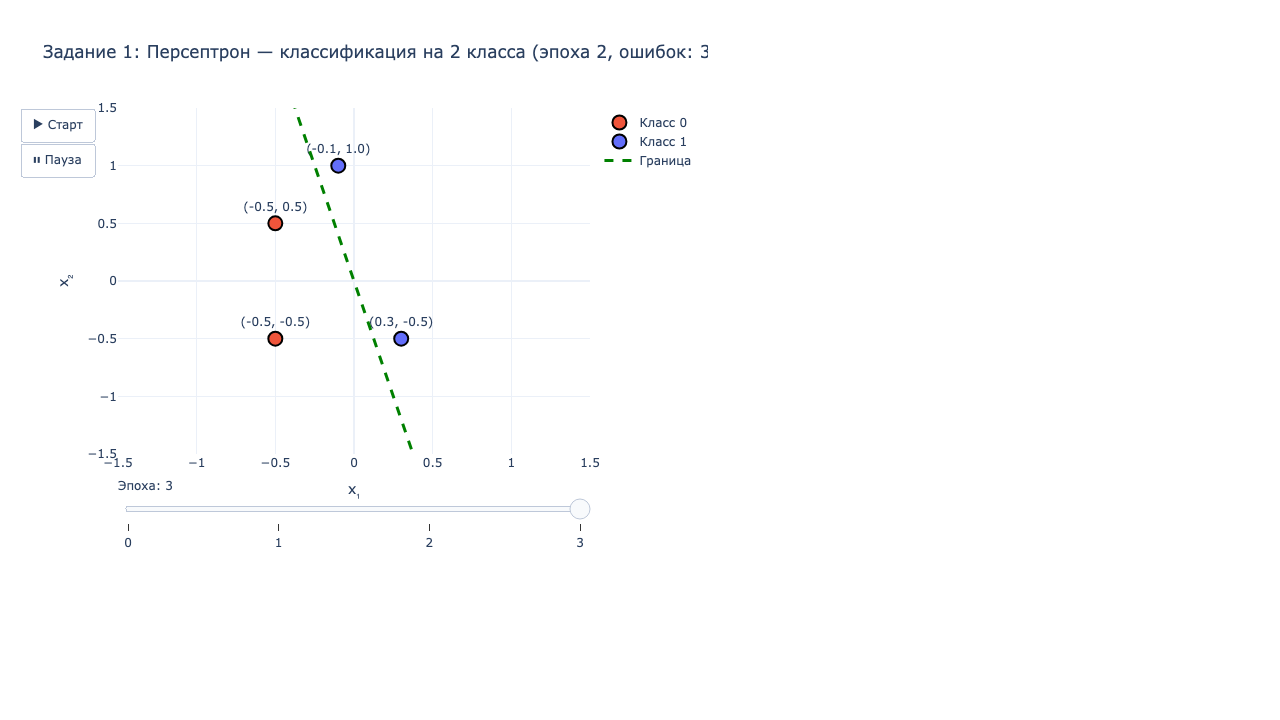
\includegraphics[width=0.95\textwidth]{task1_decision_boundary.png}
\caption{Граница решения для линейно разделимой задачи бинарной классификации.}
\label{fig:lab_01_fig_1}
\end{figure}

\begin{figure}[H]
\centering
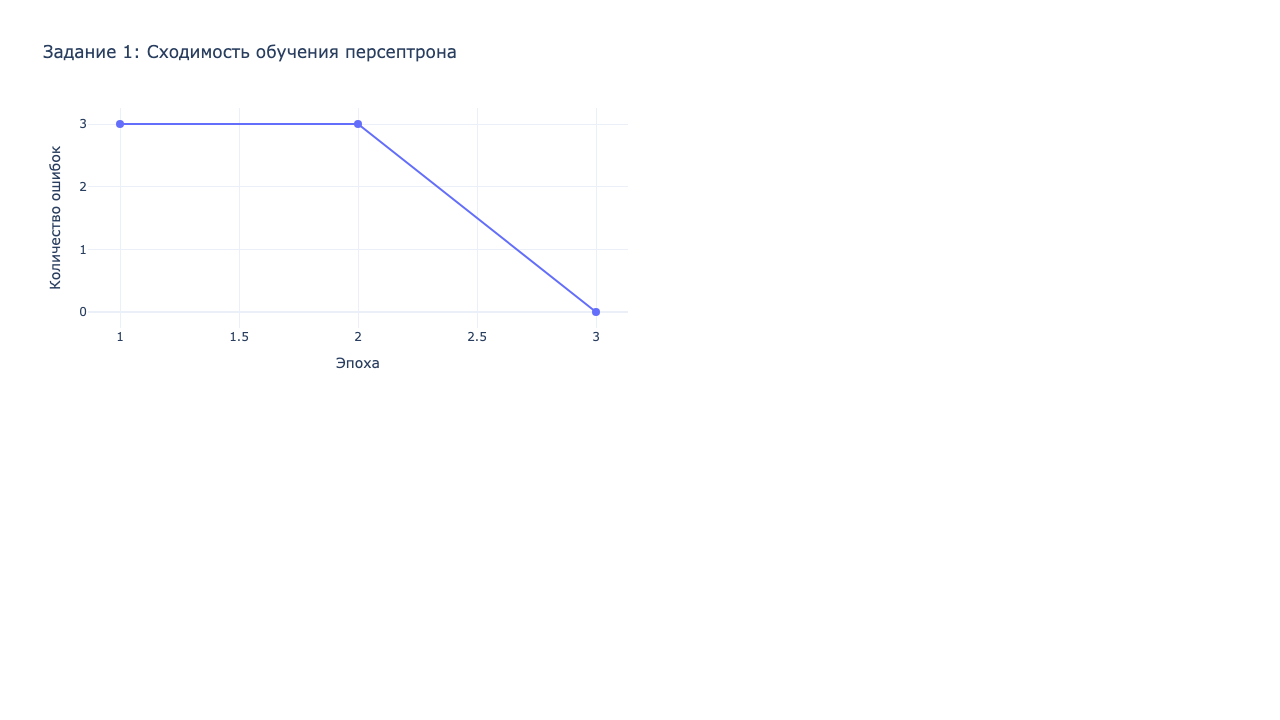
\includegraphics[width=0.95\textwidth]{task1_convergence.png}
\caption{Сходимость персептрона в задаче бинарной классификации.}
\label{fig:lab_01_fig_2}
\end{figure}

\begin{figure}[H]
\centering
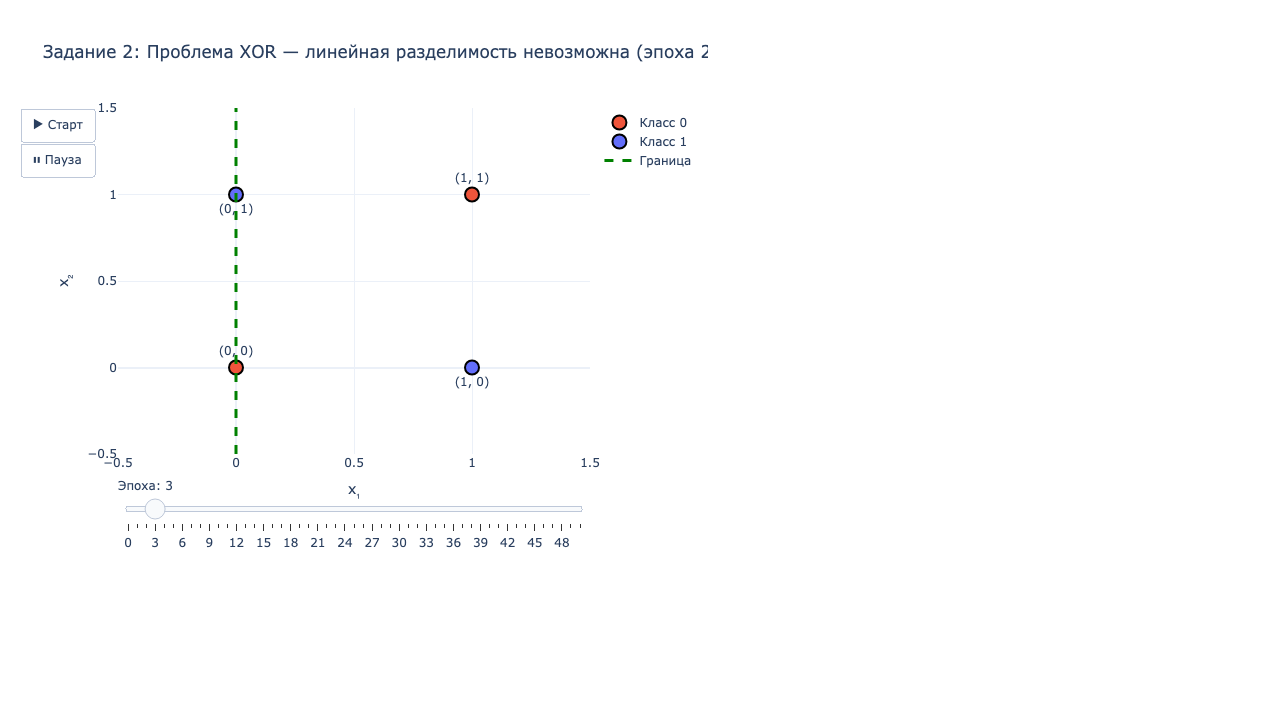
\includegraphics[width=0.95\textwidth]{task2_xor_problem.png}
\caption{Геометрическая постановка задачи XOR на плоскости.}
\label{fig:lab_01_fig_3}
\end{figure}

\begin{figure}[H]
\centering
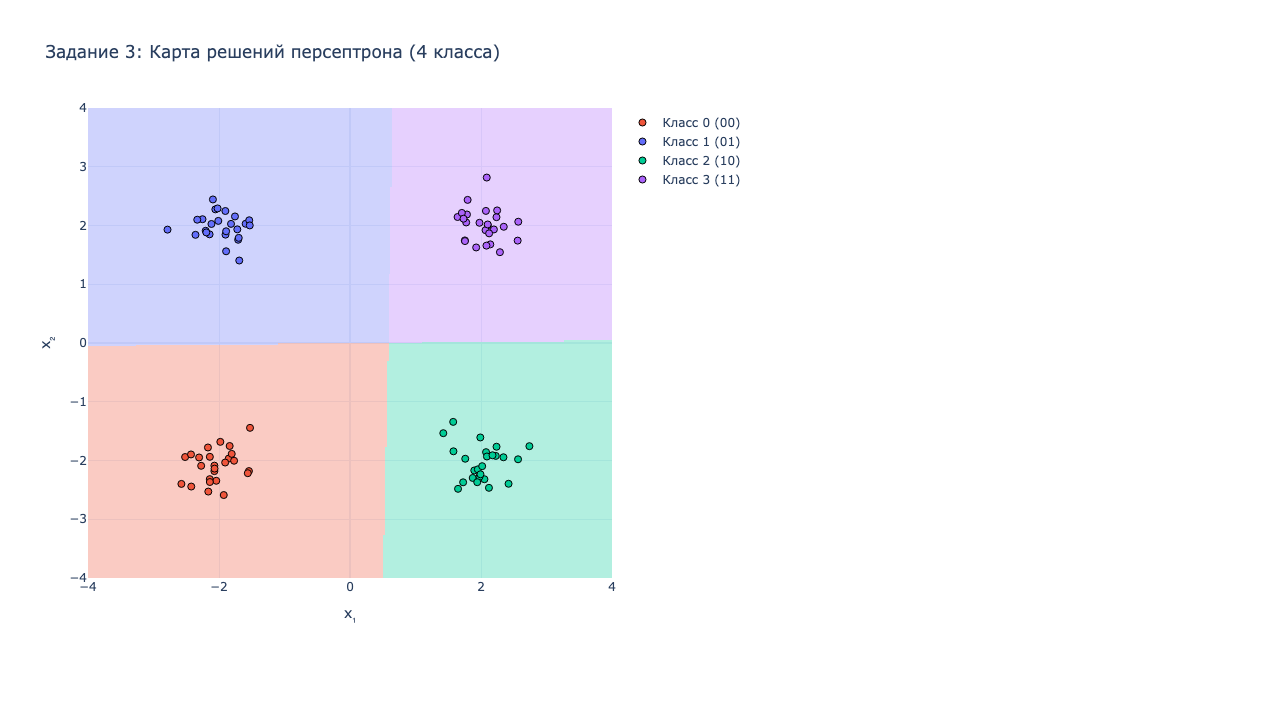
\includegraphics[width=0.95\textwidth]{task3_decision_map.png}
\caption{Карта решений персептрона из двух нейронов для четырех классов.}
\label{fig:lab_01_fig_4}
\end{figure}


\section{Выводы}

В ходе лабораторной работы изучены принципы работы и обучения персептрона. Экспериментальные результаты подтвердили теоретические положения: теорему о сходимости персептрона для линейно разделимых данных и невозможность решения задачи XOR однослойной архитектурой. Многонейронный персептрон позволяет решать задачи с большим числом классов, формируя несколько разделяющих границ.

\section{Контрольные вопросы для Moodle}

Ниже приведены 30 вопросов в форме, удобной для визуальной проверки. Исходный банк вопросов для загрузки в Moodle сохранен отдельно в файле \texttt{questions.gift.txt}.

\small
\begin{enumerate}[label=\textbf{\arabic*.}, leftmargin=0pt, itemsep=1.2em]
\item Что такое персептрон?
\begin{itemize}[label=$\square$, leftmargin=1.5cm, itemsep=0.2em, topsep=0.3em]
\item Многослойная нейронная сеть со скрытыми слоями
\item Простейшая модель искусственного нейрона, предложенная Фрэнком Розенблаттом
\item Алгоритм кластеризации данных
\item Метод понижения размерности
\end{itemize}
{\small\textit{Правильный ответ: Простейшая модель искусственного нейрона, предложенная Фрэнком Розенблаттом.}}

\item Какую задачу изначально был призван решать классический персептрон?
\begin{itemize}[label=$\square$, leftmargin=1.5cm, itemsep=0.2em, topsep=0.3em]
\item Регрессию
\item Кластеризацию
\item Бинарную классификацию
\item Прогнозирование временных рядов
\end{itemize}
{\small\textit{Правильный ответ: Бинарную классификацию.}}

\item Какую функцию активации обычно используют в классическом однослойном персептроне для классификации?
\begin{itemize}[label=$\square$, leftmargin=1.5cm, itemsep=0.2em, topsep=0.3em]
\item Сигмоиду
\item Гиперболический тангенс
\item Пороговую (единичную ступенчатую) функцию
\item ReLU
\end{itemize}
{\small\textit{Правильный ответ: Пороговую (единичную ступенчатую) функцию.}}

\item Что означает весовой коэффициент в модели нейрона?
\begin{itemize}[label=$\square$, leftmargin=1.5cm, itemsep=0.2em, topsep=0.3em]
\item Скорость обучения нейронной сети
\item Важность соответствующего входного сигнала
\item Порог срабатывания функции активации
\item Ошибку сети
\end{itemize}
{\small\textit{Правильный ответ: Важность соответствующего входного сигнала.}}

\item Для чего в персептроне используется смещение (bias)?
\begin{itemize}[label=$\square$, leftmargin=1.5cm, itemsep=0.2em, topsep=0.3em]
\item Для сдвига функции активации по оси абсцисс
\item Для изменения крутизны функции активации
\item Для уменьшения размерности входных данных
\item Для регуляризации весов
\end{itemize}
{\small\textit{Правильный ответ: Для сдвига функции активации по оси абсцисс.}}

\item В чем заключается правило обновления весов персептрона?
\begin{itemize}[label=$\square$, leftmargin=1.5cm, itemsep=0.2em, topsep=0.3em]
\item Веса изменяются пропорционально второй производной ошибки
\item Веса изменяются в направлении градиента функции потерь
\item Веса изменяются только в случае неправильной классификации примера
\item Веса случайным образом переинициализируются
\end{itemize}
{\small\textit{Правильный ответ: Веса изменяются только в случае неправильной классификации примера.}}

\item Какой параметр задает размер шага при обновлении весов?
\begin{itemize}[label=$\square$, leftmargin=1.5cm, itemsep=0.2em, topsep=0.3em]
\item Эпоха
\item Смещение
\item Коэффициент скорости обучения (learning rate)
\item Порог
\end{itemize}
{\small\textit{Правильный ответ: Коэффициент скорости обучения (learning rate).}}

\item Что такое эпоха в контексте обучения персептрона?
\begin{itemize}[label=$\square$, leftmargin=1.5cm, itemsep=0.2em, topsep=0.3em]
\item Один проход алгоритма обучения по одной случайной выборке
\item Один полный проход алгоритма обучения по всему обучающему набору данных
\item Время до остановки алгоритма
\item Момент инициализации весов
\end{itemize}
{\small\textit{Правильный ответ: Один полный проход алгоритма обучения по всему обучающему набору данных.}}

\item Какую проблему не может решить классический однослойный персептрон?
\begin{itemize}[label=$\square$, leftmargin=1.5cm, itemsep=0.2em, topsep=0.3em]
\item Логическое И (AND)
\item Логическое ИЛИ (OR)
\item Логическое исключающее ИЛИ (XOR)
\item Логическое НЕ (NOT)
\end{itemize}
{\small\textit{Правильный ответ: Логическое исключающее ИЛИ (XOR).}}

\item При каком условии однослойный персептрон гарантированно сходится (находит решение)?
\begin{itemize}[label=$\square$, leftmargin=1.5cm, itemsep=0.2em, topsep=0.3em]
\item Если обучающая выборка линейно разделима
\item Если размерность данных больше объема выборки
\item Если используется сигмоидная функция активации
\item Если скорость обучения равна нулю
\end{itemize}
{\small\textit{Правильный ответ: Если обучающая выборка линейно разделима.}}

\item Как математически можно описать границу принятия решений однослойного персептрона?
\begin{itemize}[label=$\square$, leftmargin=1.5cm, itemsep=0.2em, topsep=0.3em]
\item Полином второй степени
\item Гиперплоскость
\item Сфера
\item Эллипсоид
\end{itemize}
{\small\textit{Правильный ответ: Гиперплоскость.}}

\item Что означает линейная разделимость двух классов?
\begin{itemize}[label=$\square$, leftmargin=1.5cm, itemsep=0.2em, topsep=0.3em]
\item Классы можно разделить некоторой прямой, плоскостью или гиперплоскостью
\item Классы можно разделить только нелинейной функцией
\item Объекты обоих классов лежат на одной прямой
\item Расстояние между классами вычисляется по евклидовой метрике
\end{itemize}
{\small\textit{Правильный ответ: Классы можно разделить некоторой прямой, плоскостью или гиперплоскостью.}}

\item В случае, если классы линейно неразделимы, что произойдет при обучении классического персептрона без ограничения числа эпох?
\begin{itemize}[label=$\square$, leftmargin=1.5cm, itemsep=0.2em, topsep=0.3em]
\item Он быстро найдет нелинейную границу
\item Обучение будет длиться бесконечно, так как ошибка никогда не станет нулевой
\item Веса станут равными нулю
\item Сеть перейдет в спящий режим
\end{itemize}
{\small\textit{Правильный ответ: Обучение будет длиться бесконечно, так как ошибка никогда не станет нулевой.}}

\item К какому типу задач машинного обучения относится обучение персептрона?
\begin{itemize}[label=$\square$, leftmargin=1.5cm, itemsep=0.2em, topsep=0.3em]
\item Обучение без учителя (Unsupervised Learning)
\item Обучение с учителем (Supervised Learning)
\item Обучение с подкреплением (Reinforcement Learning)
\item Генеративное моделирование
\end{itemize}
{\small\textit{Правильный ответ: Обучение с учителем (Supervised Learning).}}

\item Как в матричном виде вычисляется взвешенная сумма для одного примера x и вектора весов w?
\begin{itemize}[label=$\square$, leftmargin=1.5cm, itemsep=0.2em, topsep=0.3em]
\item Извлечение квадратного корня из произведения
\item Векторное (скалярное) произведение x и w
\item Поэлементное деление x на w
\item Умножение матриц x и обратной к w
\end{itemize}
{\small\textit{Правильный ответ: Векторное (скалярное) произведение x и w.}}

\item Для чего необходимо добавлять фиктивный признак (обычно равный 1) к обучающим примерам при реализации персептрона?
\begin{itemize}[label=$\square$, leftmargin=1.5cm, itemsep=0.2em, topsep=0.3em]
\item Чтобы избежать нулевых значений во входных данных
\item Чтобы учесть параметр смещения (bias) в виде еще одного веса
\item Чтобы увеличить размерность пространства для лучшей разделимости
\item Для нормализации данных
\end{itemize}
{\small\textit{Правильный ответ: Чтобы учесть параметр смещения (bias) в виде еще одного веса.}}

\item Какой метод нормализации чаще всего применяется перед обучением персептрона, чтобы предотвратить доминирование признаков с большими значениями?
\begin{itemize}[label=$\square$, leftmargin=1.5cm, itemsep=0.2em, topsep=0.3em]
\item Min-Max масштабирование или Z-нормализация
\item Удаление дисперсии
\item Дискретизация
\item Лемматизация
\end{itemize}
{\small\textit{Правильный ответ: Min-Max масштабирование или Z-нормализация.}}

\item Если выход персептрона (после пороговой функции) равен 1, а истинное значение (target) равно 0, какова будет ошибка?
\begin{itemize}[label=$\square$, leftmargin=1.5cm, itemsep=0.2em, topsep=0.3em]
\item 1
\item -1
\item 0
\item 0.5
\end{itemize}
{\small\textit{Правильный ответ: -1.}}

\item Если прогноз персептрона совпадает с истинным значением, как изменятся веса?
\begin{itemize}[label=$\square$, leftmargin=1.5cm, itemsep=0.2em, topsep=0.3em]
\item Веса увеличатся на скорость обучения
\item Веса уменьшатся на скорость обучения
\item Веса останутся без изменений
\item Веса обнулятся
\end{itemize}
{\small\textit{Правильный ответ: Веса останутся без изменений.}}

\item Зачем случайным образом инициализируются веса перед началом обучения?
\begin{itemize}[label=$\square$, leftmargin=1.5cm, itemsep=0.2em, topsep=0.3em]
\item Чтобы гарантировать сходимость за одну эпоху
\item Чтобы нарушить симметрию, если выходов несколько, и задать начальную точку поиска
\item Чтобы персептрон всегда давал разные ответы
\item Это не обязательно, всегда можно начать с единиц
\end{itemize}
{\small\textit{Правильный ответ: Чтобы нарушить симметрию, если выходов несколько, и задать начальную точку поиска.}}

\item Может ли персептрон с двумя входами решать задачу классификации на три класса?
\begin{itemize}[label=$\square$, leftmargin=1.5cm, itemsep=0.2em, topsep=0.3em]
\item Да, один нейрон легко решает многоклассовую задачу
\item Нет, один классический персептрон выполняет только бинарную классификацию
\item Да, если использовать линейную функцию активации
\item Да, если увеличить скорость обучения
\end{itemize}
{\small\textit{Правильный ответ: Нет, один классический персептрон выполняет только бинарную классификацию.}}

\item Какой подход позволяет классифицировать несколько классов с помощью персептронов?
\begin{itemize}[label=$\square$, leftmargin=1.5cm, itemsep=0.2em, topsep=0.3em]
\item Один против всех (One-vs-All)
\item Метод главных компонент
\item Деревья решений
\item Случайный лес
\end{itemize}
{\small\textit{Правильный ответ: Один против всех (One-vs-All).}}

\item Чем обусловлена необходимость выбора небольшой, но не нулевой скорости обучения?
\begin{itemize}[label=$\square$, leftmargin=1.5cm, itemsep=0.2em, topsep=0.3em]
\item Нулевая не обновляет веса, а слишком большая может приводить к расхождению (проскок оптимума)
\item Ограничениями памяти компьютера
\item Ограничениями вычислительных ресурсов компьютера
\item Чтобы веса всегда становились отрицательными
\end{itemize}
{\small\textit{Правильный ответ: Нулевая не обновляет веса, а слишком большая может приводить к расхождению (проскок оптимума).}}

\item Каким образом происходит остановка алгоритма обучения персептрона на практике?
\begin{itemize}[label=$\square$, leftmargin=1.5cm, itemsep=0.2em, topsep=0.3em]
\item Только когда ошибка становится нулевой
\item При достижении нулевой ошибки или максимального заданного числа эпох
\item После первой эпохи
\item Когда веса превышают 100
\end{itemize}
{\small\textit{Правильный ответ: При достижении нулевой ошибки или максимального заданного числа эпох.}}

\item Какой ученый доказал ограниченность однослойного персептрона в решении задачи XOR?
\begin{itemize}[label=$\square$, leftmargin=1.5cm, itemsep=0.2em, topsep=0.3em]
\item Фрэнк Розенблатт
\item Марвин Минский и Сеймур Паперт
\item Уоррен МакКаллок
\item Артур Сэмюэл
\end{itemize}
{\small\textit{Правильный ответ: Марвин Минский и Сеймур Паперт.}}

\item Что вернет пороговая функция Хевисайда, если взвешенная сумма равна 2.5 (порог активации = 0)?
\begin{itemize}[label=$\square$, leftmargin=1.5cm, itemsep=0.2em, topsep=0.3em]
\item 0
\item 1
\item 2.5
\item -1
\end{itemize}
{\small\textit{Правильный ответ: 1.}}

\item Можно ли использовать градиентный спуск для настройки весов в классическом персептроне со ступенчатой функцией активации?
\begin{itemize}[label=$\square$, leftmargin=1.5cm, itemsep=0.2em, topsep=0.3em]
\item Да, ступенчатая функция везде дифференцируема
\item Нет, производная ступенчатой функции равна нулю почти везде, градиентный спуск не применим
\item Да, но только при скорости обучения больше 1
\item Да, с использованием метода вторых производных
\end{itemize}
{\small\textit{Правильный ответ: Нет, производная ступенчатой функции равна нулю почти везде, градиентный спуск не применим.}}

\item Как оценивается качество классификации персептроном на тестовой выборке?
\begin{itemize}[label=$\square$, leftmargin=1.5cm, itemsep=0.2em, topsep=0.3em]
\item С помощью метрики Среднеквадратичная ошибка (MSE)
\item С помощью доли правильных ответов (Accuracy)
\item С помощью R-квадрат
\item Через псевдообратную матрицу
\end{itemize}
{\small\textit{Правильный ответ: С помощью доли правильных ответов (Accuracy).}}

\item Что геометрически представляет собой вектор весов обученного персептрона по отношению к разделяющей гиперплоскости?
\begin{itemize}[label=$\square$, leftmargin=1.5cm, itemsep=0.2em, topsep=0.3em]
\item Касательную к разделяющей гиперплоскости
\item Нормаль (перпендикуляр) к разделяющей гиперплоскости
\item Точку на гиперплоскости
\item Не имеет геометрической интерпретации
\end{itemize}
{\small\textit{Правильный ответ: Нормаль (перпендикуляр) к разделяющей гиперплоскости.}}

\item Какая теорема гарантирует, что алгоритм обучения персептрона найдет разделяющую гиперплоскость за конечное число шагов при условии линейной разделимости классов?
\begin{itemize}[label=$\square$, leftmargin=1.5cm, itemsep=0.2em, topsep=0.3em]
\item Теорема Байеса
\item Теорема сходимости персептрона (Perceptron Convergence Theorem)
\item Теорема о среднем значении
\item Центральная предельная теорема
\end{itemize}
{\small\textit{Правильный ответ: Теорема сходимости персептрона (Perceptron Convergence Theorem).}}

\end{enumerate}



\end{document}
